\makeatletter
\def\input@path{{../styles/}{../../styles/}{../../../styles/}{../}{../../}{../../../}}
\makeatother
\documentclass{ee102_notes}
% macros.tex - Course meta information
\renewcommand{\course}{EE 102}
\renewcommand{\coursetitle}{Signal Processing and Linear Systems}
\renewcommand{\instructor}{Ayush Pandey}
\renewcommand{\semester}{Fall}
\renewcommand{\year}{2025}
\renewcommand{\shorttitle}{Week 1: Introduction to Signals}
% Use \renewcommand to avoid 'already defined' errors

% The following packages can be found on http:\\www.ctan.org
% \usepackage{graphics} % for pdf, bitmapped graphics files
%\usepackage{epsfig} % for postscript graphics files
%\usepackage{mathptmx} % assumes new font selection scheme installed
%\usepackage{times} % assumes new font selection scheme installed
\usepackage{amsmath} % assumes amsmath package installed
\usepackage{amssymb,mathtools}  % assumes amsmath package installed
\usepackage{xcolor}
\usepackage{pgfplots,subcaption}
\usepackage[hidelinks]{hyperref}
\usepackage{verbatim}
\usepackage{graphicx}
\usepackage{listings}

% -------- listings (Python) ----------
\lstdefinestyle{py}{
  language=Python,
  basicstyle=\ttfamily\small,
  keywordstyle=\color{blue!60!black}\bfseries,
  commentstyle=\color{green!40!black},
  stringstyle=\color{orange!60!black},
  showstringspaces=false,
  columns=fullflexible,
  frame=single,
  framerule=0.3pt,
  numbers=left,
  numberstyle=\tiny,
  xleftmargin=1em,
  tabsize=2,
  breaklines=true,
}
\usepackage[american]{circuitikz}
\usepackage{tikz}
\usepackage{caption}    
\usepackage{lscape}
\usepackage{soul}
\usepackage{tikz}
\usetikzlibrary{calc,angles,quotes,arrows.meta}

\usepackage{hyperref}
\hypersetup{
    colorlinks=true,
    linkcolor=blue,
    filecolor=magenta,      
    urlcolor=blue,
    pdftitle={week1_notes},
    pdfpagemode=FullScreen,
}
%\usepackage{float} 

%\usepackage[demo]{graphicx}
\pgfplotsset{compat=1.18}
% \usepgfplotslibrary{fillbetween}

\newsavebox{\measurebox}

\let\proof\relax\let\endproof\relax


\newcommand{\norm}[1]{\left\lVert#1\right\rVert}
\def\abs#1{\left\lvert#1\right\rvert}
\let\proof\relax
\let\endproof\relax
\usepackage{amsthm}
\usepackage{accents}
\usepackage{relsize}
\newcommand{\ubar}[1]{\underaccent{\bar}{#1}}
\newtheorem{theorem}{Theorem}
\newtheorem{corollary}{Corollary}[theorem]
\newtheorem{lemma}{Lemma}
\newtheorem{proposition}{Proposition}
\newtheorem{statement}{Statement}

\theoremstyle{definition}
\newtheorem{definition}{Definition}
 
\theoremstyle{remark}
\newtheorem*{remark}{Remark}
\theoremstyle{remark}
\newtheorem*{claim}{Claim}
\setlength{\parindent}{0cm}
\newenvironment{nalign}{
    \begin{equation}
    \begin{aligned}
}{
    \end{aligned}
    \end{equation}
    \ignorespacesafterend
}

\usetikzlibrary{arrows.meta,calc}
\renewcommand{\releasedate}{September 15, 2025}
\sisetup{per-mode=symbol,retain-explicit-plus}

\newcommand{\Eblank}{\rule{3cm}{0.4pt}}
\newcommand{\Rankblank}{\rule{3cm}{0.4pt}}

\begin{document}

\section*{EE 102 Week 3, Lecture 1 (Fall 2025)}
\subsection*{Instructor: \instructor}
\subsection*{Date: \releasedate}

\section*{Logistics}
\begin{itemize}
  \item HW \#3 due: Mon, Sep 22 (new deadlines: every Monday at midnight). \quad Midterm: Wed, Sep 24.
  \item Feedback from Week 2: new assignment deadline, more worked examples, will tie to book exercises, and the weekly HW. 
  \item New office hours (Ayush): Mondays at 3.30pm in the library cafe. (Yaoyun, TBD): Fridays at 12pm. 
  \item Midterm exam: in class, closed book, timed. One hour exam. Will be designed to be completed in 40 minutes. Will cover material up to Week 3 Lecture 2. A practice quiz will be posted on CatCourses. No programming problems on the exam.
  \item Suggested study approach (in order): lecture notes, concepts on the HW assignments, books as references (work on solved examples). 
\end{itemize}

\section{Goals for today}
We will review EE 102 topics so far. This includes: signals, sketching signals, properties of signals, transformations of signals, and the three special signals (step, impulse, complex exponentials).

\section{Icebreaker activity: comparing signal energy}
You are driving an electric vehicle (EV) on a one-hour trip from point A to point B. There are many ways you can do this trip --- which one uses the least energy?
\medskip

\noindent Each team is assigned a simple signal trace \(x(t)\)  that represents how much battery is used up in an electric vehicle over \([0,1]\) hour for a given scenario (assume arbitrary units such that the math works out). Your task is to compute the total energy \(E\) (in \si{kWh}) to determine who has the biggest energy consumption and predict your rank (1 = least energy spent). Among your team, you should confirm that everyone has the same answer and come to a consensus of the rank. Then, you will be asked to announce your energy and your guess of where you stand.

\medskip

\textbf{Key formula (use \(t\) in hours):}
\[
E  = \int_{-\infty}^{\infty} |x(t)|^2 \,dt.
\]

\bigskip
\hrule
\bigskip

\section*{Team Prompts (pick one per team)}
All signals are zero outside the intervals shown.

\subsection*{Team 1: Flat road, stop, flat road}
\[
x_1(t)=
\begin{cases}
12, & 0 \le t < \tfrac{1}{3} \\
0, & \tfrac{1}{3} \le t < \tfrac{2}{3} \\
12, & \tfrac{2}{3} \le t \le 1 \\
0, & \text{otherwise}
\end{cases}
\]
\begin{tcolorbox}[title=Team 1: Record your results]
Energy \(E=\) \Eblank\ \si{kWh} \quad\quad Predicted rank \(=\) \Rankblank\ (/8)
\end{tcolorbox}

\subsection*{Team 2: Uphill, stop, downhill}
\[
x_2(t)=
\begin{cases}
18, & 0 \le t < \tfrac{1}{3} \quad\text{(uphill)}\\
0,  & \tfrac{1}{3} \le t < \tfrac{2}{3} \quad\text{(stop)}\\
6,  & \tfrac{2}{3} \le t \le 1 \quad\text{(downhill)}\\
0,  & \text{otherwise}
\end{cases}
\]
\begin{tcolorbox}[title=Team 2: Record your results]
Energy \(E=\) \Eblank\ \si{kWh} \quad\quad Predicted rank \(=\) \Rankblank\ (/8)
\end{tcolorbox}

\subsection*{Team 3: Rapid cruise (less efficient) to destination}
\[
x_3(t)=
\begin{cases}
13.5, & 0 \le t < \tfrac{2}{3} \\
0,    & \tfrac{2}{3} \le t \le 1 \\
0,    & \text{otherwise}
\end{cases}
\]
\begin{tcolorbox}[title=Team 3: Record your results]
Energy \(E=\) \Eblank\ \si{kWh} \quad\quad Predicted rank \(=\) \Rankblank\ (/8)
\end{tcolorbox}

\subsection*{Team 4: Dynamic speeding (ramp up, then ramp down)}
Ramp up such that battery uses from 8 to 16 over the first \SI{0.5}{h}, then ramp down to 8 over the next \SI{0.5}{h}.
\[
x_4(t)=
\begin{cases}
8 + 16\,t, & 0 \le t < \tfrac{1}{2} \\
24 - 16\,t, & \tfrac{1}{2} \le t \le 1 \\
0, & \text{otherwise}
\end{cases}
\]
\begin{tcolorbox}[title=Team 4: Record your results]
Energy \(E=\) \Eblank\ \si{kWh} \quad\quad Predicted rank \(=\) \Rankblank\ (/8)
\end{tcolorbox}

\subsection*{Team 5: Stop-and-go traffic (three bursts)}
Scenario where $x(t) = 18$ for three \SI{10}{min} segments, with \SI{10}{min} stops between.
\[
x_5(t)=
\begin{cases}
18, & 0 \le t < \tfrac{1}{6}, \;\;\tfrac{1}{3}\le t < \tfrac{1}{2}, \;\;\tfrac{2}{3}\le t < \tfrac{5}{6} \\
0,  & \text{else on }[0,1]\\
0,  & \text{otherwise}
\end{cases}
\]
\begin{tcolorbox}[title=Team 5: Record your results]
Energy \(E=\) \Eblank\ \si{kWh} \quad\quad Predicted rank \(=\) \Rankblank\ (/8)
\end{tcolorbox}

\subsection*{Team 6: Eco mode (slow and steady)}
\[
x_6(t)=
\begin{cases}
9, & 0 \le t \le 1 \\
0, & \text{otherwise}
\end{cases}
\]
\begin{tcolorbox}[title=Team 6: Record your results]
Energy \(E=\) \Eblank\ \si{kWh} \quad\quad Predicted rank \(=\) \Rankblank\ (/8)
\end{tcolorbox}

\subsection*{Team 7: Late starter, speeding later}
\[
x_7(t)=
\begin{cases}
0, & 0 \le t < \tfrac{1}{2} \\
16, & \tfrac{1}{2} \le t \le 1 \\
0, & \text{otherwise}
\end{cases}
\]
\begin{tcolorbox}[title=Team 7: Record your results]
Energy \(E=\) \Eblank\ \si{kWh} \quad\quad Predicted rank \(=\) \Rankblank\ (/8)
\end{tcolorbox}

\subsection*{Team 8 — Two hills then cruise}
\[
P_8(t)=
\begin{cases}
24, & 0 \le t < \tfrac{1}{4} \\
6,  & \tfrac{1}{4} \le t < \tfrac{1}{2} \\
10, & \tfrac{1}{2} \le t \le 1 \\
0,  & \text{otherwise}
\end{cases}
\]
\begin{tcolorbox}[title=Team 8: Record your results]
Energy \(E=\) \Eblank\ \si{kWh} \quad\quad Predicted rank \(=\) \Rankblank\ (/8)
\end{tcolorbox}
\newpage

\section{Review: signals and basic properties}
Refer to the previous week's notes for more details on signals. As a quick reminder: we defined signals as mathematical functions that describe physical quantities or represent information. 
\subsection{Basic properties of signals}
\begin{itemize}
  \item \textbf{Continuous-time and discrete-time:} Continuous-time signals are defined for every real-valued time \(t\), while discrete time signals are defined only at discrete time instances \(n\) (usually integers).
  \item \textbf{Energy and power signals:} Energy signals have finite energy \[E = \int_{-\infty}^{\infty} |x(t)|^2 dt < \infty\] and zero average power, while power signals have finite, non-zero average power \[P = \lim_{T \to \infty} \frac{1}{2T} \int_{-T}^{T} |x(t)|^2 dt < \infty\] and infinite energy.
  \item \textbf{Deterministic and random signals:} Deterministic signals can be precisely described by mathematical functions, while random signals exhibit uncertainty and are often characterized statistically.
  \item \textbf{Periodicity} Periodic signals repeat after a fixed interval \(T\) (i.e., \(x(t) = x(t+T)\)), while aperiodic signals do not exhibit such repetition. The smallest time-shift $T_0$ for which \(x(t) = x(t+T_0)\) is called the fundamental period.
  \item \textbf{Even vs. odd:} Even signals satisfy \(x(t) = x(-t)\), while odd signals satisfy \(x(t) = -x(-t)\).
\end{itemize}
\subsection{Signal transformations}
Remember that the two most important types of transformations are time shifts and time scaling: 
\[
y(t) = x(t - t_0) \quad \text{(time shift)}, \qquad y(t) = x(a t) \quad \text{(time scaling)}.
\]
Here, for time-shift the $t$ is replaced by $t - t_0$, and for time-scaling the $t$ is replaced by $a t$. So, if the signal is $x(t) = A\sin(\omega t + \phi)$, then the time-shifted signal is $y(t) = A\sin(\omega (t - t_0) + \phi)$ and the time-scaled signal is $y(t) = A\sin(\omega (a t) + \phi)$. 
\subsection{Decomposition of signals with even and odd functions}
In this course, we will often decompose signals into its fundamental components. There are many ways in which you can define these components. One of these is decomposing a signal into an even and an odd part. This helps us apply the properties of even and odd functions to analyze the signal, without having to analyze the entire signal at once.

Consider a signal $x(t)$,
\[
x(t) = x_{\text{e}}(t) + x_{\text{o}}(t),\qquad
x_{\text{e}}(t) \triangleq \frac{x(t)+x(-t)}{2},\quad
x_{\text{o}}(t) \triangleq \frac{x(t)-x(-t)}{2}.
\]

\paragraph{Pop quiz}
Show that $x_{\text{e}}(t)$ is an even function and $x_{\text{o}}(t)$ is an odd function.


\section{The ``timeless trio'' of signals}
We noted three special signals: step, impulse, complex exponential and gave them a name (the ``timeless trio''). We will now review these three signals in more detail.
\
\subsection{The unit step as a switch}
The unit step $u(t)$ is a fundamental building block for constructing piecewise signals. It acts as a switch that turns on at \(t=0\) and remains on thereafter. By combining and shifting unit steps, we can create complex piecewise functions.

The ideal unit step function is not realizable in practice. However, smooth \emph{sigmoids} can approximate $u(t)$. You will find that these sigmoids are the main building blocks of neural networks! In a reductionist view, neural networks are just millions (or billions) of such sigmoids (unit steps) trained together to approximate any general function. That's why neural networks are sometimes also called \emph{universal function approximators}. Someone who learns signal processing will be able to see the deeper picture: everything is a switch after all (as in electronics and computers).

You can write down the sigmoid functions as approximate unit steps:
\[
\sigma_k(t) \;=\; \frac{1}{1+e^{-k t}}
\quad\text{and}\quad
\tilde\sigma_k(t) \;=\; \frac{1}{2}\!\left(1+\tanh(kt)\right),
\qquad k\gg 1 \Rightarrow \sigma_k(t)\approx u(t).
\]

Let's consider two examples to demonstrate the power of the unit step functions. 
\subsection{Example 1: A square wave using steps}
 The bipolar square pulse in Figure~\ref{fig:steps-square} can be written as a combination of unit step functions. Let's try to build it step-by-step. First, note that the first unit step (part 1 of the figure) turns on the signal at $t=0$, so this can be written as $u(t)$. Next, we want the signal to turn off at $t=1$ (part 2 of the figure). Consider the time-shifted signal $u(t-1)$, which turns on at $t=1$. If we subtract this from the first step, we get a signal that is $+1$ on $[0,T)$ and $0$ elsewhere. Next, we want the signal to turn negative at $t=2T$ (part 3 of the figure). Consider the negative of the step function $-u(t-2T)$, which turns on at $t=2T$. Adding this to the previous result gives a signal that is $+1$ on $[0,T)$, $0$ on $[T,2T)$, and $-1$ on $[2T,\infty)$. Finally, we want the signal to return to $0$ at $t=3T$ (part 4 of the figure). Consider the time-shifted step $u(t-3T)$, which turns on at $t=3T$. Adding this to the previous result gives the desired square pulse. Thus, the complete expression for the square pulse is
\[
x(t) \;=\; u(t)-u(t-T)\;-\;u(t-2T)+u(t-3T)
\]
equals $+1$ on $[0,T)$, $0$ on $[T,2T)$, $-1$ on $[2T,3T)$, and $0$ otherwise.
It is a sum of four shifted/scaled steps. Figure~\ref{fig:steps-square} overlays the four contributors.

\begin{figure}[h!]
\centering
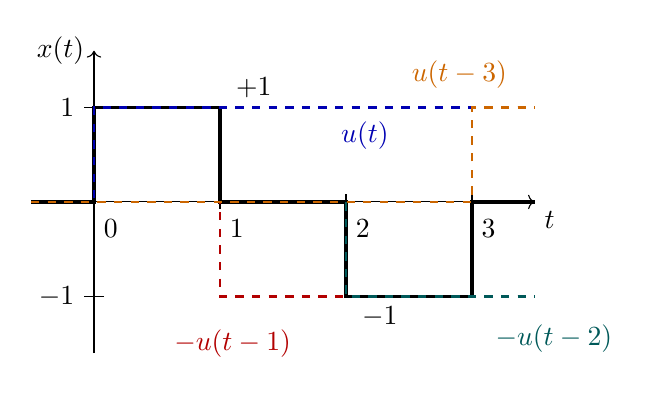
\begin{tikzpicture}[x=1.6cm,y=1.2cm]
  \def\xmin{-0.5} \def\xmax{3.5}
  \def\ymin{-1.6} \def\ymax{1.6}

  % axes
  \draw[->] (\xmin,0) -- (\xmax,0) node[below right] {$t$};
  \draw[->] (0,\ymin) -- (0,\ymax) node[left] {$x(t)$};

  % tick marks, move x ticks towards right.
  \foreach \t in {0,1,2,3}
    \draw (\t,0.08) -- (\t,-0.08) node[below right] {$\t$};
  \foreach \y in {-1,1}
    \draw (0.08,\y) -- (-0.08,\y) node[left] {$\y$};

  % composite square pulse
  \draw[line width=1.2pt]
    (\xmin,0) -- (0,0) -- (0,1) -- (1,1) -- (1,0) -- (2,0) -- (2,-1) -- (3,-1) -- (3,0) -- (\xmax,0);
  \node[above right] at (1.05,1) {$+1$};
  \node[below right] at (2.05,-1) {$-1$};

  % colored contributors (scaled steps)
  % + u(t)
  \draw[blue!70!black, dashed, line width=1pt]
    (\xmin,0) -- (0,0) -- (0,1) -- (\xmax,1);
  \node[blue!70!black] at (2.15,0.7) {$u(t)$};

  % - u(t-1)
  \draw[red!70!black, dashed, line width=1pt]
    (\xmin,0) -- (1,0) -- (1,-1) -- (\xmax,-1);
  \node[red!70!black] at (1.1,-1.5) {$-u(t-1)$};

  % - u(t-2)
  \draw[teal!70!black, dashed, line width=1pt]
    (\xmin,0) -- (2,0) -- (2,-1) -- (\xmax,-1);
  \node[teal!70!black] at (3.65,-1.45) {$-u(t-2)$};

  % + u(t-3)
  \draw[orange!80!black, dashed, line width=1pt]
    (\xmin,0) -- (3,0) -- (3,1) -- (\xmax,1);
  \node[orange!80!black] at (2.9,1.35) {$u(t-3)$};

  % braces to indicate segments
%   \draw[decorate,decoration={brace,amplitude=6pt},yshift=6pt] (0,1.05) -- (1,1.05) node[midway, yshift=8pt] {$+1$};
%   \draw[decorate,decoration={brace,amplitude=6pt,mirror},yshift=-6pt] (2,-1.05) -- (3,-1.05) node[midway, yshift=-10pt] {$-1$};
\end{tikzpicture}
\caption{Square pulse constructed as $u(t)-u(t-T)-u(t-2T)+u(t-3T)$ (here $T=1$). Colored dashed curves show the four step contributors.}
\label{fig:steps-square}
\end{figure}

\paragraph{Example 2 (piecewise levels using steps).}
A signal that is $0$ for $t<1$, jumps to $1$ on $[1,2)$, and then to $2$ for $t\ge 2$ can be written \emph{only} with steps:
\[
x(t) \;=\; u(t-1) + u(t-2).
\]
More generally, any piecewise-constant $x(t)$ can be expressed as $\sum_k a_k\,u(t-t_k)$ with appropriate increments $a_k$ at the change points $t_k$.

\subsection{The unit impulse as a sampler}
We defined the impulse by its sifting property:
\[
\int_{-\infty}^{\infty} f(t)\,\delta(t-t_0)\,dt \;=\; f(t_0).
\]
Think of $\delta$ as an idealized sampler that extracts the value of $f(t)$ at $t_0$.

A common approximation uses a narrow rectangle (area $1$):
\[
p_\varepsilon(t)\;=\;\frac{1}{\varepsilon}\Big[u\!\left(t+\tfrac{\varepsilon}{2}\right)-u\!\left(t-\tfrac{\varepsilon}{2}\right)\Big],
\qquad \lim_{\varepsilon\to 0^+} p_\varepsilon(t) = \delta(t)\;\; \text{in the distribution sense.}
\]
You can visualize this approximation by running the \href{https://github.com/ee-ucmerced/ee102-signals-systems/blob/main/lecture\_notes/week2\_signal\_properties/VM_delta_via_pulse.py}{{\tt VM\_delta\_via\_pulse.py}} script available on course Github.

\subsection{Complex exponentials}
We have discussed the complex exponential function before: $e^{j\omega t}$. However, that is just a special case of the generalized complex exponential
\[
x(t) \;=\; A e^{s t}, \qquad A\in\mathbb{C},\;\; s=\sigma + j\omega \in \mathbb{C}.
\]
\paragraph{Why complex numbers / complex signals?} 

With complex numbers, the central question is always: why did we even introduce the imaginary! Recall that when we worked with 2D vectors, we could represent them instead using a complex scalar. So, the vector operations, which can be tricky to account for become simpler with the standard scalar algebra that is applicable for complex numbers. We want the same convenience with signals. Additionally, as we will see, complex exponentials let us represent a \emph{really} large class of signals such as sinusoids (of all kinds!), exponentials (both growing and decaying), and arbitrary combinations of these!

\begin{popquiz} Recall that the utility of complex numbers is that they allow us to represent higher dimensions, in this case, two signals, using just one signal. Can you identify the two signals represented by $x(t) = e^{j\omega t}$?
    \popquizsolution{The two signals are the real and imaginary parts of the complex exponential: $\Re\{x(t)\} = \cos(\omega t)$ and $\Im\{x(t)\} = \sin(\omega t)$.}
\end{popquiz}
To see that the general complex exponential can represent a large class of signals, write $A = |A|e^{j\phi}$ to obtain the \emph{amplitude-phase} form
\[
x(t) \;=\; |A|\,e^{\sigma t}\,e^{j(\omega t + \phi)}
\;=\; e^{\sigma t}\Big(|A|\cos(\omega t+\phi) \;+\; j\,|A|\sin(\omega t+\phi)\Big).
\]
Special cases emerge by selecting $A$ and $s$:

\paragraph{1. A sinusoidal signal (pick $A$ and $s$):}
Set $\sigma=0$, $A=|A|e^{j\phi}$, $s=j\omega$:
\[
x(t) = |A|e^{j(\omega t+\phi)} \;\Rightarrow\;
\Re\{x(t)\} = |A|\cos(\omega t+\phi),\;\; \Im\{x(t)\}=|A|\sin(\omega t+\phi).
\]
You can see that $e^{j\omega t}$ is periodic with $T=\tfrac{2\pi}{\omega}$ for $\omega\neq 0$.

\begin{popquiz} When is $A e^{s t}$ a constant $k$?
    \popquizsolution{Set $\omega=0$ and $\sigma=0$ to get $x(t)=A=k$. For real $k$, choose $A\in\mathbb{R}$.}
\end{popquiz}
\paragraph{2. Real decaying exponential:}
Take $\omega=0$, $\sigma<0$, and $A\in\mathbb{R}$:
\[
x(t)=A e^{\sigma t},\quad \text{monotone decay to $0$ as $t\to\infty$.}
\]
\begin{popquiz} Derive the growing exponential using the complex exponential.
    \popquizsolution{Set $\sigma>0$, $\omega=0$, and $A\in\mathbb{R}$ to get $x(t)=A e^{\sigma t}$, which grows unbounded as $t\to\infty$.}
\end{popquiz}

\paragraph{3. Exponentially damped sinusoid.}
Choose $\sigma<0$, $\omega\neq 0$, $A=|A|e^{j\phi}$ and take the real part:
\[
x(t)=|A|e^{\sigma t}\cos(\omega t+\phi).
\]
\begin{popquiz} Derive the exponentially growing cosine using the complex exponential.
    \popquizsolution[4]{Set $\sigma>0$, $\omega\neq 0$, and $A=|A|e^{j\phi}$ to get $x(t)=|A|e^{\sigma t}\cos(\omega t+\phi)$, which grows unbounded as $t\to\infty$.}
\end{popquiz}
\subsubsection{Using complex algebra}
You can derive all of the standard signals above from the general complex exponential also by expanding out the complex exponential by writing $A = a_1 + j b_1$ and $s = \sigma + j\omega$:
\[
x(t) = (a_1 + j b_1) e^{(\sigma + j\omega) t} = (a_1 + j b_1) e^{\sigma t} (\cos(\omega t) + j \sin(\omega t)).
\]
Expanding this out, we get
\[
x(t) = e^{\sigma t} \big( (a_1 \cos(\omega t) - b_1 \sin(\omega t)) + j (a_1 \sin(\omega t) + b_1 \cos(\omega t)) \big).
\]
Thus, the real and imaginary parts of $x(t)$ are
\[
\Re\{x(t)\} = e^{\sigma t} (a_1 \cos(\omega t) - b_1 \sin(\omega t)), \quad \Im\{x(t)\} = e^{\sigma t} (a_1 \sin(\omega t) + b_1 \cos(\omega t)).
\]
This shows that by choosing appropriate values for $a_1$, $b_1$, $\sigma$, and $\omega$, we can generate a wide variety of signals, including sinusoids, exponentials, and combinations thereof.
\section*{Next steps}
Next class: properties of systems (time invariance, linearity, causality, memory/memoryless, invertibility), responses of LTI systems, and how complex exponentials act as eigenfunctions of LTI systems.

\end{document}
